%%%%%%%%%%%%%%%%%%%%%%%%%%%%%%%%%%%%
% This is the template for submission to ISCA 2016
% The cls file is a modified from  'sig-alternate.cls'
%%%%%%%%%%%%%%%%%%%%%%%%%%%%%%%%%%%%

\documentclass{sig-alternate} 
\usepackage{mathptmx} % This is Times font

\newcommand{\ignore}[1]{}
\usepackage{fancyhdr}
\usepackage[normalem]{ulem}
\usepackage[hyphens]{url}
\usepackage{hyperref}


%%%%%%%%%%%---SETME-----%%%%%%%%%%%%%
\newcommand{\hpcasubmissionnumber}{NaN}
%%%%%%%%%%%%%%%%%%%%%%%%%%%%%%%%%%%%

\fancypagestyle{firstpage}{
  \fancyhf{}
\setlength{\headheight}{50pt}
\renewcommand{\headrulewidth}{0pt}
  \fancyhead[C]{} 
  \pagenumbering{arabic}
}  

%%%%%%%%%%%---SETME-----%%%%%%%%%%%%%
\title{Extract Useful Features for Detecting Transient Faults} 
\author{Zhiqiang Sui, Zhefan Ye, Karthik Desingh}
%%%%%%%%%%%%%%%%%%%%%%%%%%%%%%%%%%%%

\begin{document}
\maketitle
\thispagestyle{firstpage}
\pagestyle{plain}

\begin{abstract}

\end{abstract}

\section{Introduction}
In this report, we present a pipeline that can inject faults into programs and analyze how injected fault can alter program outcomes. To detect transient fault has been a research topic in robust system design for years. We utilize gemFI to study how faults are going to affect programs. Our contribution is two-fold: we implemented a fault inject pipeline, and provide analysis on how to predict fault and program outcome based on a machine learning approach. Figure~\ref{fig:teaser} shows the overview of our approach.

\begin{figure}[t]
\begin{center}
   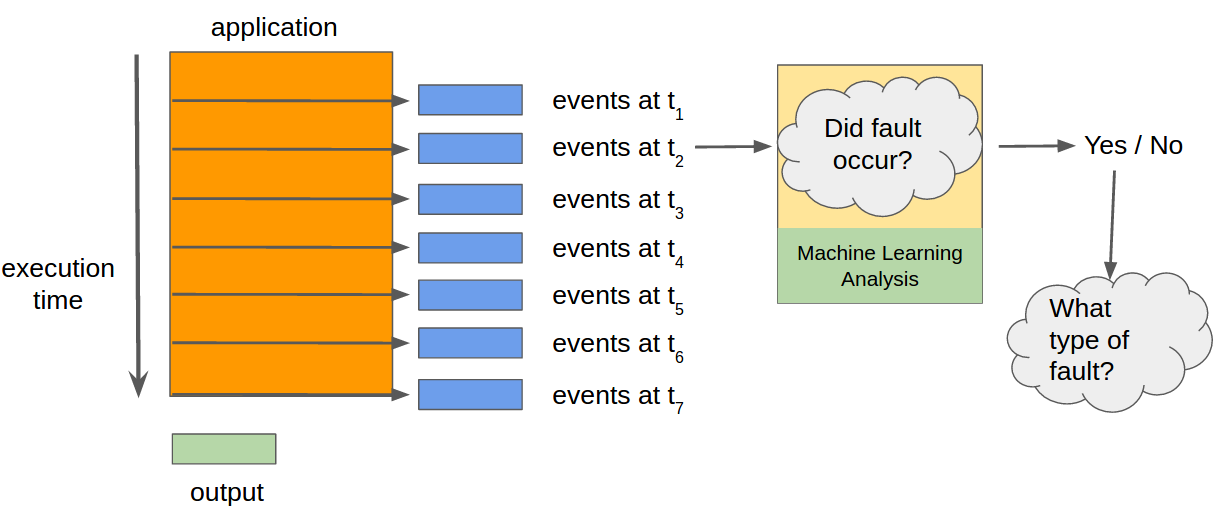
\includegraphics[width=0.95\linewidth]{./figures/teaser.png}
\end{center}
   \caption{Overview}
\label{fig:teaser}
\end{figure}

\section{Related Work}

\section{Approach}
In this section, we present our implementation for injecting faults, as well as analysis for predicting program outcome and fault types.

\subsection{Pipeline}
Figure~\ref{fig:pipeline} shows the pipeline.
\begin{figure*}[t]
\begin{center}
   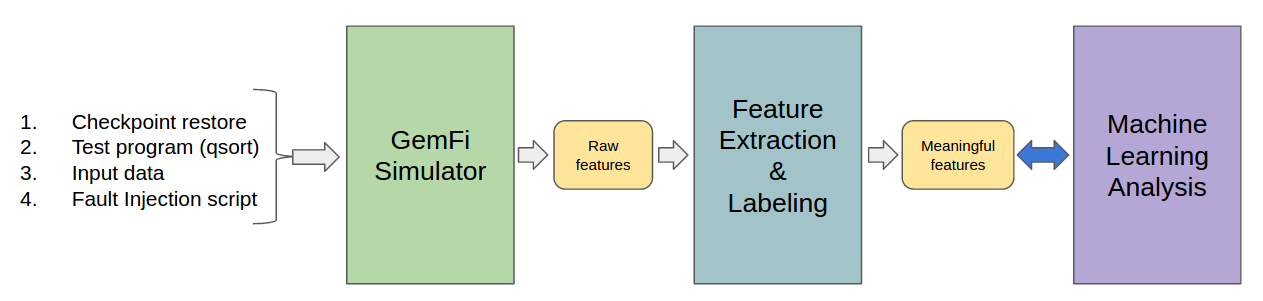
\includegraphics[width=0.95\linewidth]{./figures/pipeline.png}
\end{center}
   \caption{}
\label{fig:pipeline}
\end{figure*}

\subsection{Fault Injection}

\subsection{Feature Extraction}

\begin{figure*}[t]
\begin{center}
   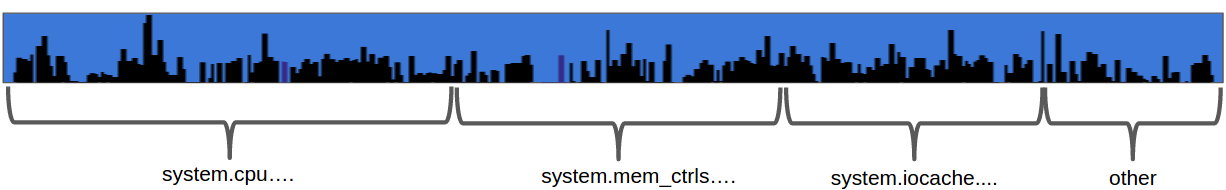
\includegraphics[width=0.95\linewidth]{./figures/feat_dist.png}
\end{center}
   \caption{}
\label{fig:feat-dist}
\end{figure*}

\subsection{Machine Analysis}
We use the random forest algorithm to predict program outcome and fault type. A random forest is essentially an ensemble of single decision trees, as illustrated in ~\ref{fig:rf} \cite{breiman2001random}. It captures different models of the data, with each decision tree representing a model, and allows us to analyze the importance of different features. 

\begin{figure}[t]
\begin{center}
   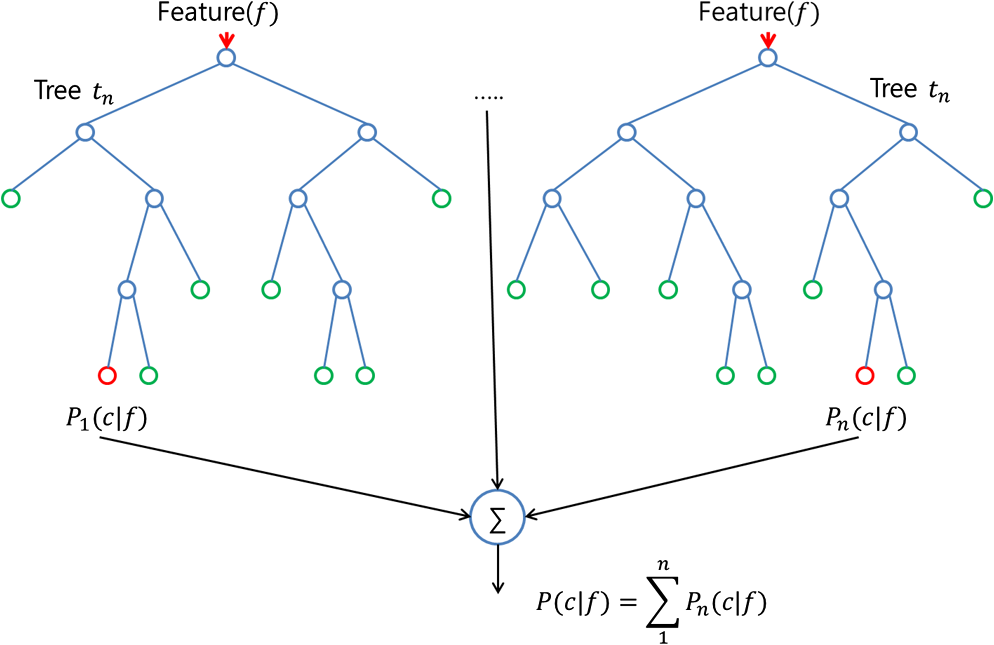
\includegraphics[width=0.95\linewidth]{./figures/rf.png}
\end{center}
   \caption{}
\label{fig:rf}
\end{figure}

\subsubsection{Training and Testing}
We randomly select $60\%$ of instances for training and $40\%$ of instances for testing. Our dataset consists of $98,000$ data instance.

\section{Experiment}

\subsection{Metrics}
we use Precision-Recall (PR) curve and $F_1$ score as our evaluation criteria. More precisely, we have
\begin{equation}
F_{1} = 2\cdot\frac{precision \cdot recall}{precision + recall},
\end{equation}
where $precision = \frac{tp}{tp+fp}$, $recall = \frac{tp}{tp+fn}$, $tp$ is the number true positive samples, $fp$ is number of false positive samples, and $fn$ is the number of false negative samples. For multi-class classification, we use confusion matrix to describe the performance of our classifier.

We design four experiment setups: 1) Experiment 1: same input data with all meaningful features, 2) Experiment 2: same sets of input data with handpicked subsets of features, 3) experiment 3: different sets of input data with all meaningful features, and 4) experiment 4: different sets of input data with handpicked subsets of features.

\subsection{Same Input All Features}
(same input all features SIAF)

\begin{figure}[t]
\begin{center}
   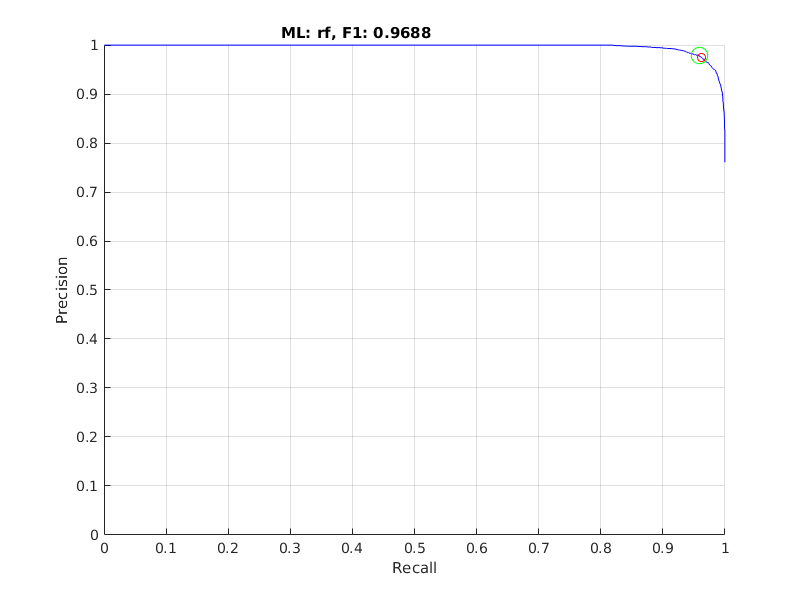
\includegraphics[width=0.95\linewidth]{./figures/siaf.png}
\end{center}
   \caption{}
\label{fig:siaf}
\end{figure}

\begin{figure}[t]
\begin{center}
   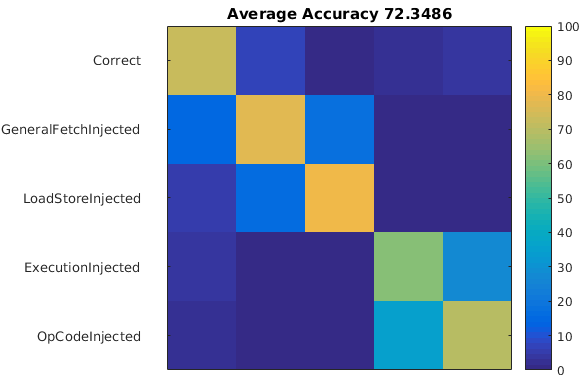
\includegraphics[width=0.95\linewidth]{./figures/siaf_multi.png}
\end{center}
   \caption{}
\label{fig:siaf-multi}
\end{figure}

The random forest algorithm output the importance score of each feature based on its discriminative power. The importance feature ranking is depicted in Figure~\ref{fig:feat-same}.
\begin{figure}[t]
\begin{center}
   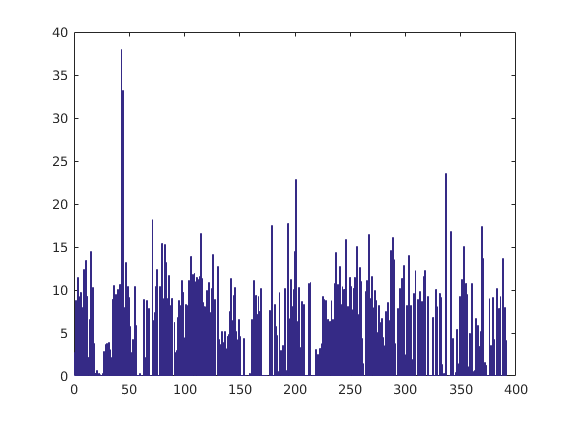
\includegraphics[width=0.95\linewidth]{./figures/feat_same.png}
\end{center}
   \caption{}
\label{fig:feat-same}
\end{figure}

\subsection{Same Input Different Features}
(same input handpicked features SIHF)

\begin{figure}[t]
\begin{center}
   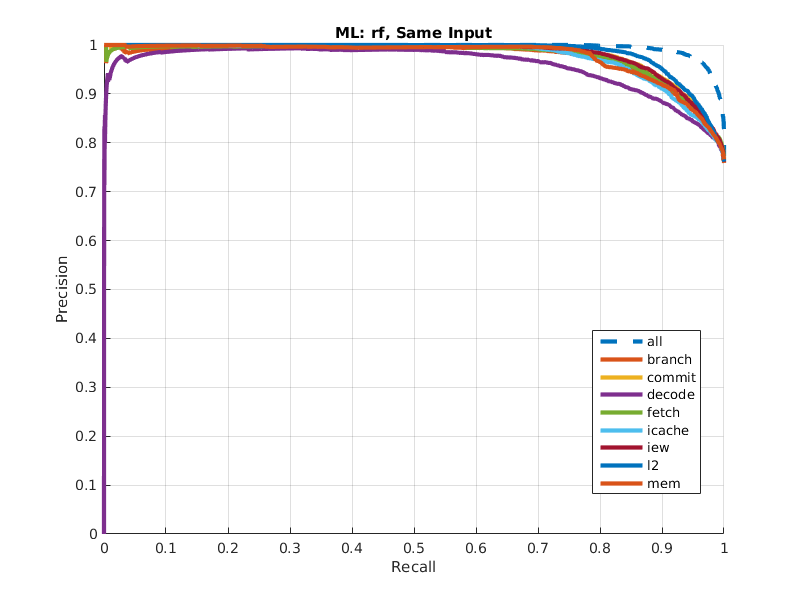
\includegraphics[width=0.95\linewidth]{./figures/sidf.png}
\end{center}
   \caption{}
\label{fig:sidf}
\end{figure}

\subsection{Different Input All Features}
(different input all features DIAF)

\begin{figure}[t]
\begin{center}
   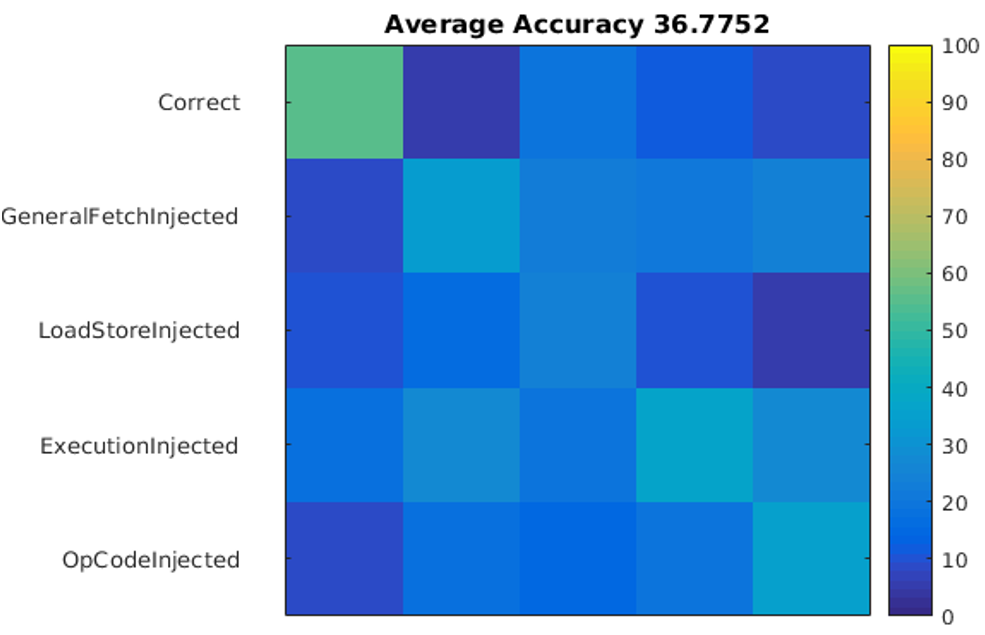
\includegraphics[width=0.95\linewidth]{./figures/diaf_multi.png}
\end{center}
   \caption{}
\label{fig:diaf-multi}
\end{figure}

\begin{figure}[t]
\begin{center}
   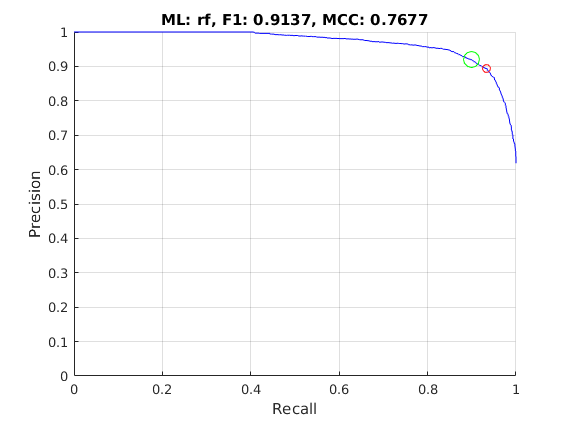
\includegraphics[width=0.95\linewidth]{./figures/disf.png}
\end{center}
   \caption{}
\label{fig:disf}
\end{figure}

\begin{figure}[t]
\begin{center}
   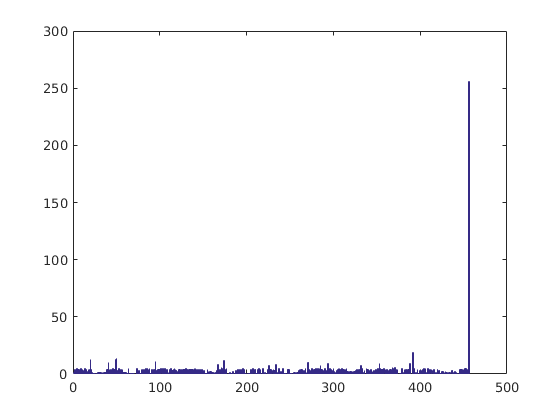
\includegraphics[width=0.95\linewidth]{./figures/feat_diff.png}
\end{center}
   \caption{}
\label{fig:feat-diff}
\end{figure}

\subsection{Different Input Different Features}
Different Input Handpicked Features DIHF

\begin{figure}[t]
\begin{center}
   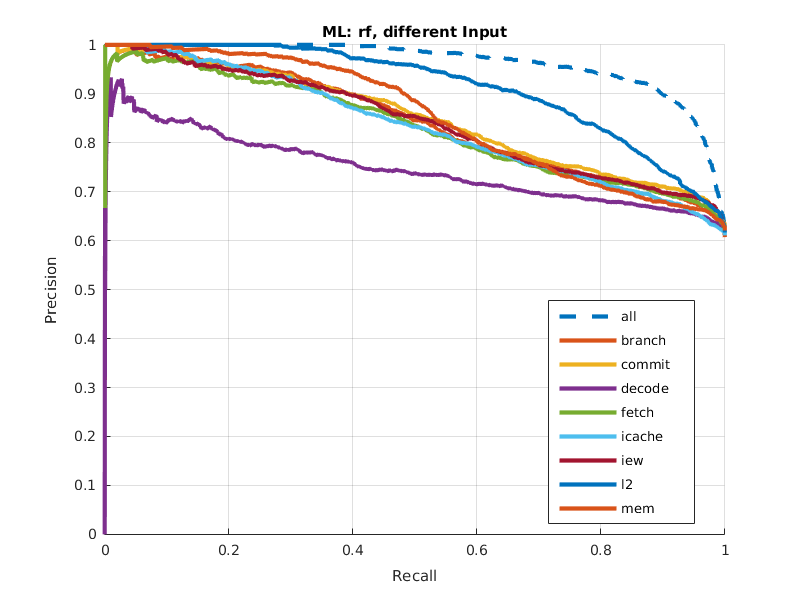
\includegraphics[width=0.95\linewidth]{./figures/didf.png}
\end{center}
   \caption{}
\label{fig:didf}
\end{figure}


\section{Discussion and Conclusion}
In the same input scenario, a few features alone can determine the results in same input condition. For same input the most important features are mainly describing the execution length. For d different input scenario: the features such as, “type of functional units issued”, “fetch instructions” and “cache read and write”, play important role in the prediction. Overall features based on “L2 cache” events perform higher than other set of hand-picked features. However, when all the features are used, the performance of the random forest algorithm is high. We extract meaningful fault signatures from the architectural events that can be used to predict transient fault occurrence.


%%%%%%% -- PAPER CONTENT ENDS -- %%%%%%%%

%%%%%%%%% -- BIB STYLE AND FILE -- %%%%%%%%
\bibliographystyle{ieeetr}
\bibliography{ref}
%%%%%%%%%%%%%%%%%%%%%%%%%%%%%%%%%%%%

\end{document}
